
\section{What is a Game?}

\begin{frame}[standout]
    \onslide<+->
    \customFigure[1]{
        
\includegraphics{Documents/250307 BIP Portorož SI/Figures/doorman.png}
    }{Someone's at the door.}{Someone's at the door.}
\end{frame}

\begin{frame}[standout]
    \onslide<+->
    \customFigure[0.42]{
        
\includegraphics{Documents/250307 BIP Portorož SI/Figures/ScrollsAndBooks_87_t.PNG}
    }{We found a book!}{We found a book!}
\end{frame}

\begin{frame}{\insertsection}
    \onslide<+->
    \blockquote[\cite{carse1986FiniteInfiniteGames}]{No one can play who is forced to play. It is an invariable principle of all play [...] that whoever plays, plays freely. Whoever must play, cannot play.}

    \vspace{2em}

    \onslide<+->
    \blockquote[\cite{carse1986FiniteInfiniteGames}]{A finite game is played for the purpose of winning, an infinite game for the purpose of continuing the play.}

    \vspace{2em}

    \onslide<+->
    \blockquote[\cite{burgun2013GameDesignTheory}]{Game: a contest of ambiguous decision making.}

    \vspace{2em}

    \onslide<+->
    \blockquote[\cite{schell2019ArtGameDesign}]{When people play games, they have an experience. It is this experience that the designer cares about. Without the experience, the game is worthless.}
\end{frame}

\begin{frame}{\insertsection}
    \onslide<+->
    \blockquote[\cite{suits1978GrasshopperGamesLife}]{The relation between playing games and winning games seems to be exhibited more generally in a class of activities which may be called 'trying and achieving' activities of a special kind; namely, where the trying and the achieving are each sought as ends in themselves. Games, it should be noticed, are not the only activities of this kind. 'It is better to have loved and lost than never to have loved at all.'}
\end{frame}

\begin{frame}[standout]
    \onslide<+->
    \customFigure[0.42]{
        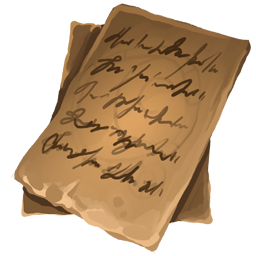
\includegraphics{Documents/250307 BIP Portorož SI/Figures/ScrollsAndBooks_102_t.PNG}
    }{A couple of pages fall out.}{A couple of pages fall out.}
\end{frame}



\subsection{Describing Play}

\begin{frame}{\insertsection\ \insertsubsection}
    \onslide<+->
    \blockquote[\cite{suits1978GrasshopperGamesLife,huizinga1964HomoLudensStudy}]{Summing up the formal characteristics of play we might call it a free activity standing quite consciously outside “ordinary” life as being “not serious,” but at the same time absorbing the player intensely and utterly. It is an activity connected with no material interest, and no profit can be gained by it. It proceeds within its own proper boundaries of time and space according to fixed rules and in an orderly manner. It promotes the formation of social groupings which tend to surround themselves with secrecy and to stress their difference from the common world by disguise or other means.}
\end{frame}



\subsection{Classifying Games}

\begin{frame}{\insertsection\ \insertsubsection}
    \onslide<+->

    \begin{multicols}{2}
        Non-comprehensive classification of games \cite{caillois2001ManPlayGames}:
    
        \begin{itemize}
            \item Ag\^{o}n -- competition
            \item Alea -- chance
            \item Mimicry -- simulation
            \item Ilinx -- vertigo
        \end{itemize}

        \columnbreak

        \begin{center}
            \onslide<2->
                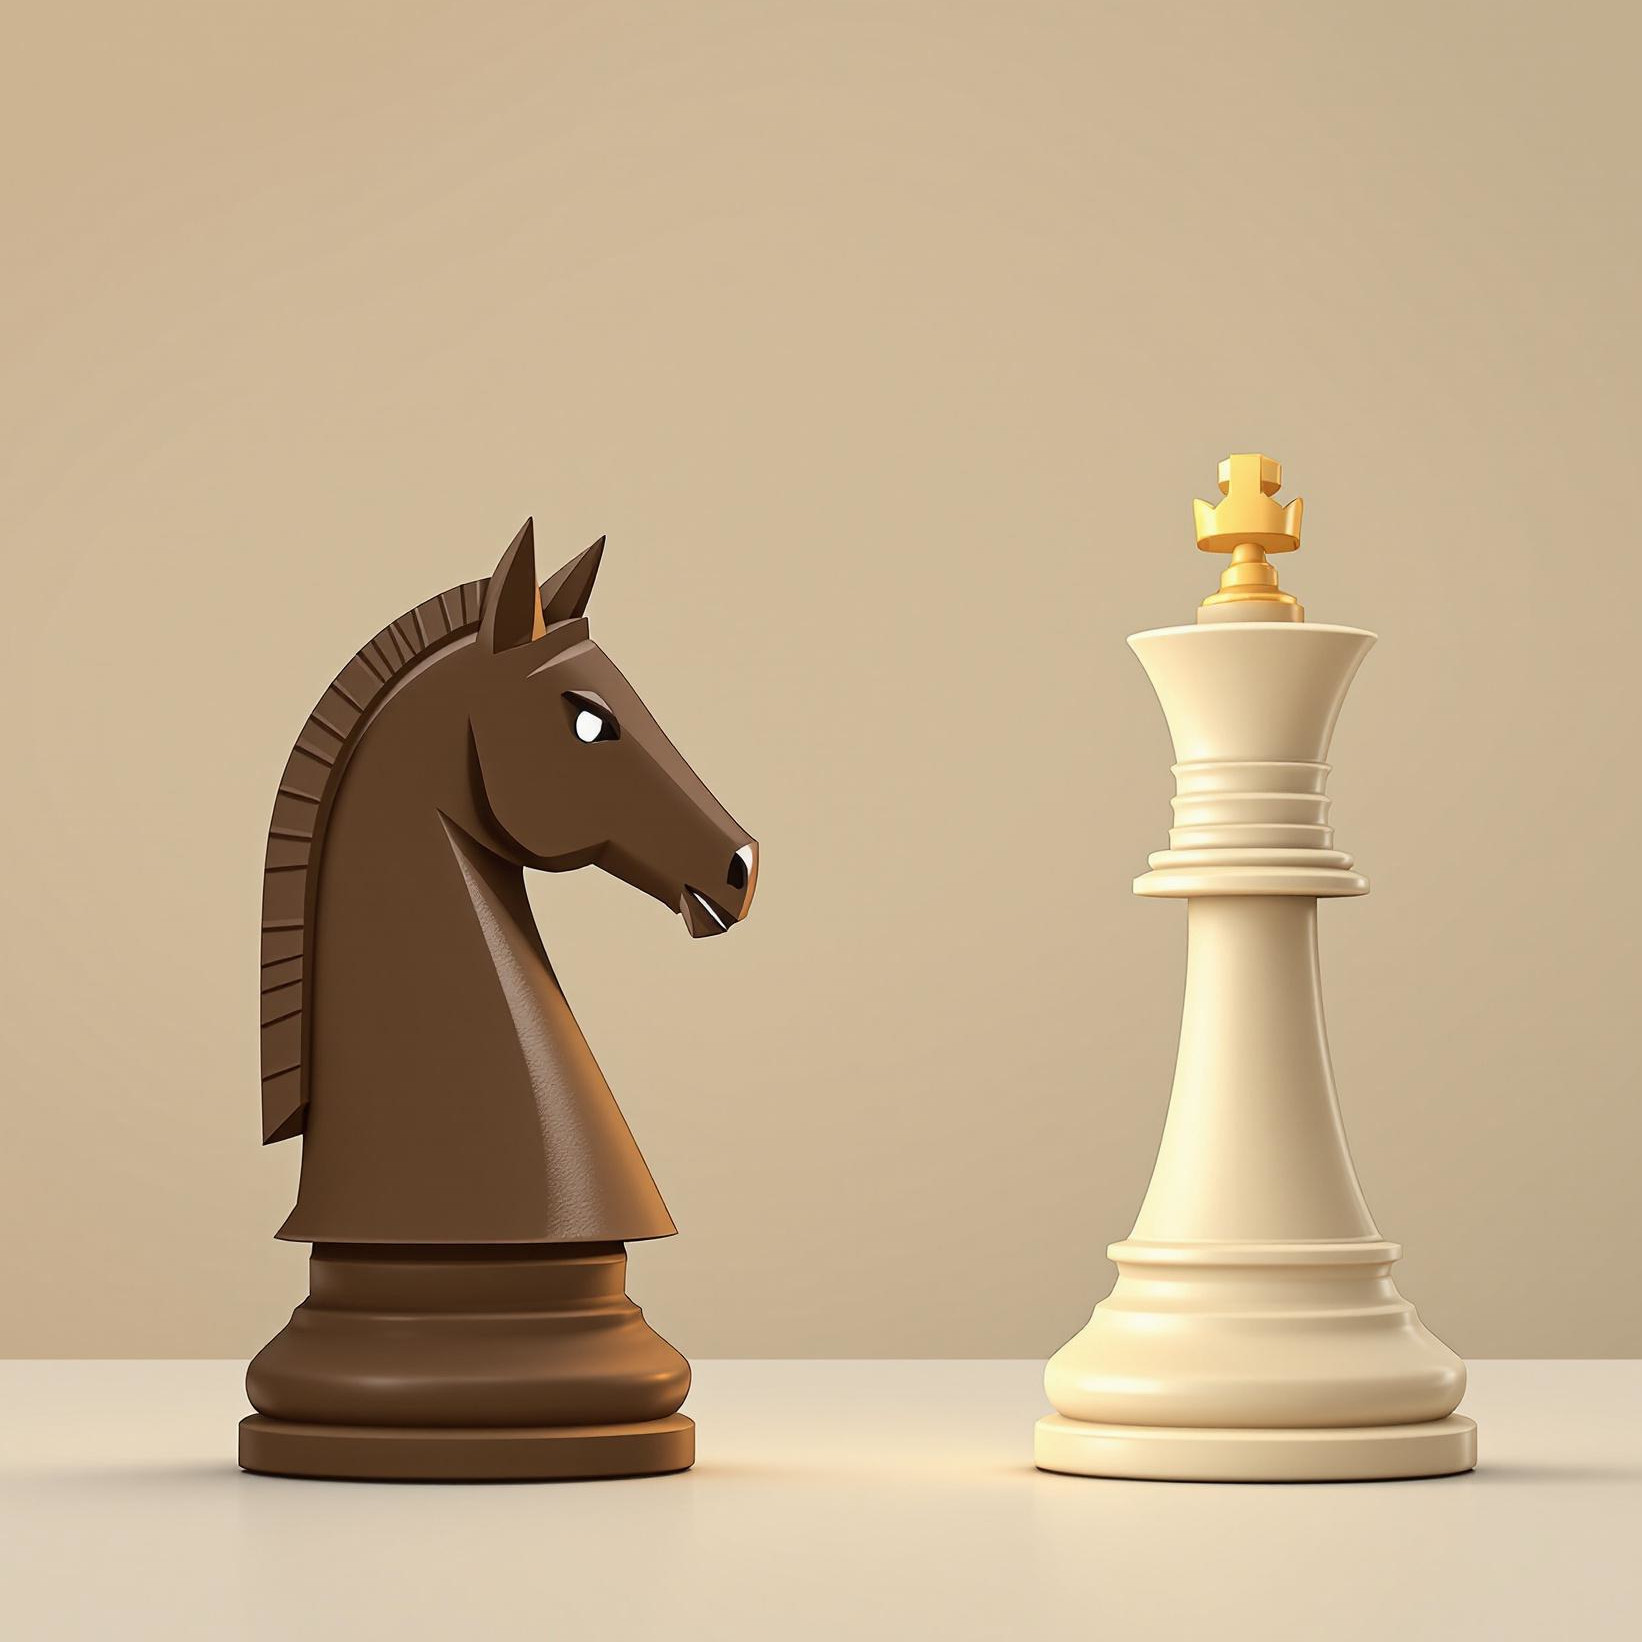
\includegraphics[width=0.4\linewidth]{Documents/250307 BIP Portorož SI/Figures/agon.jpg}
            \hspace{1em}
            \onslide<3->
                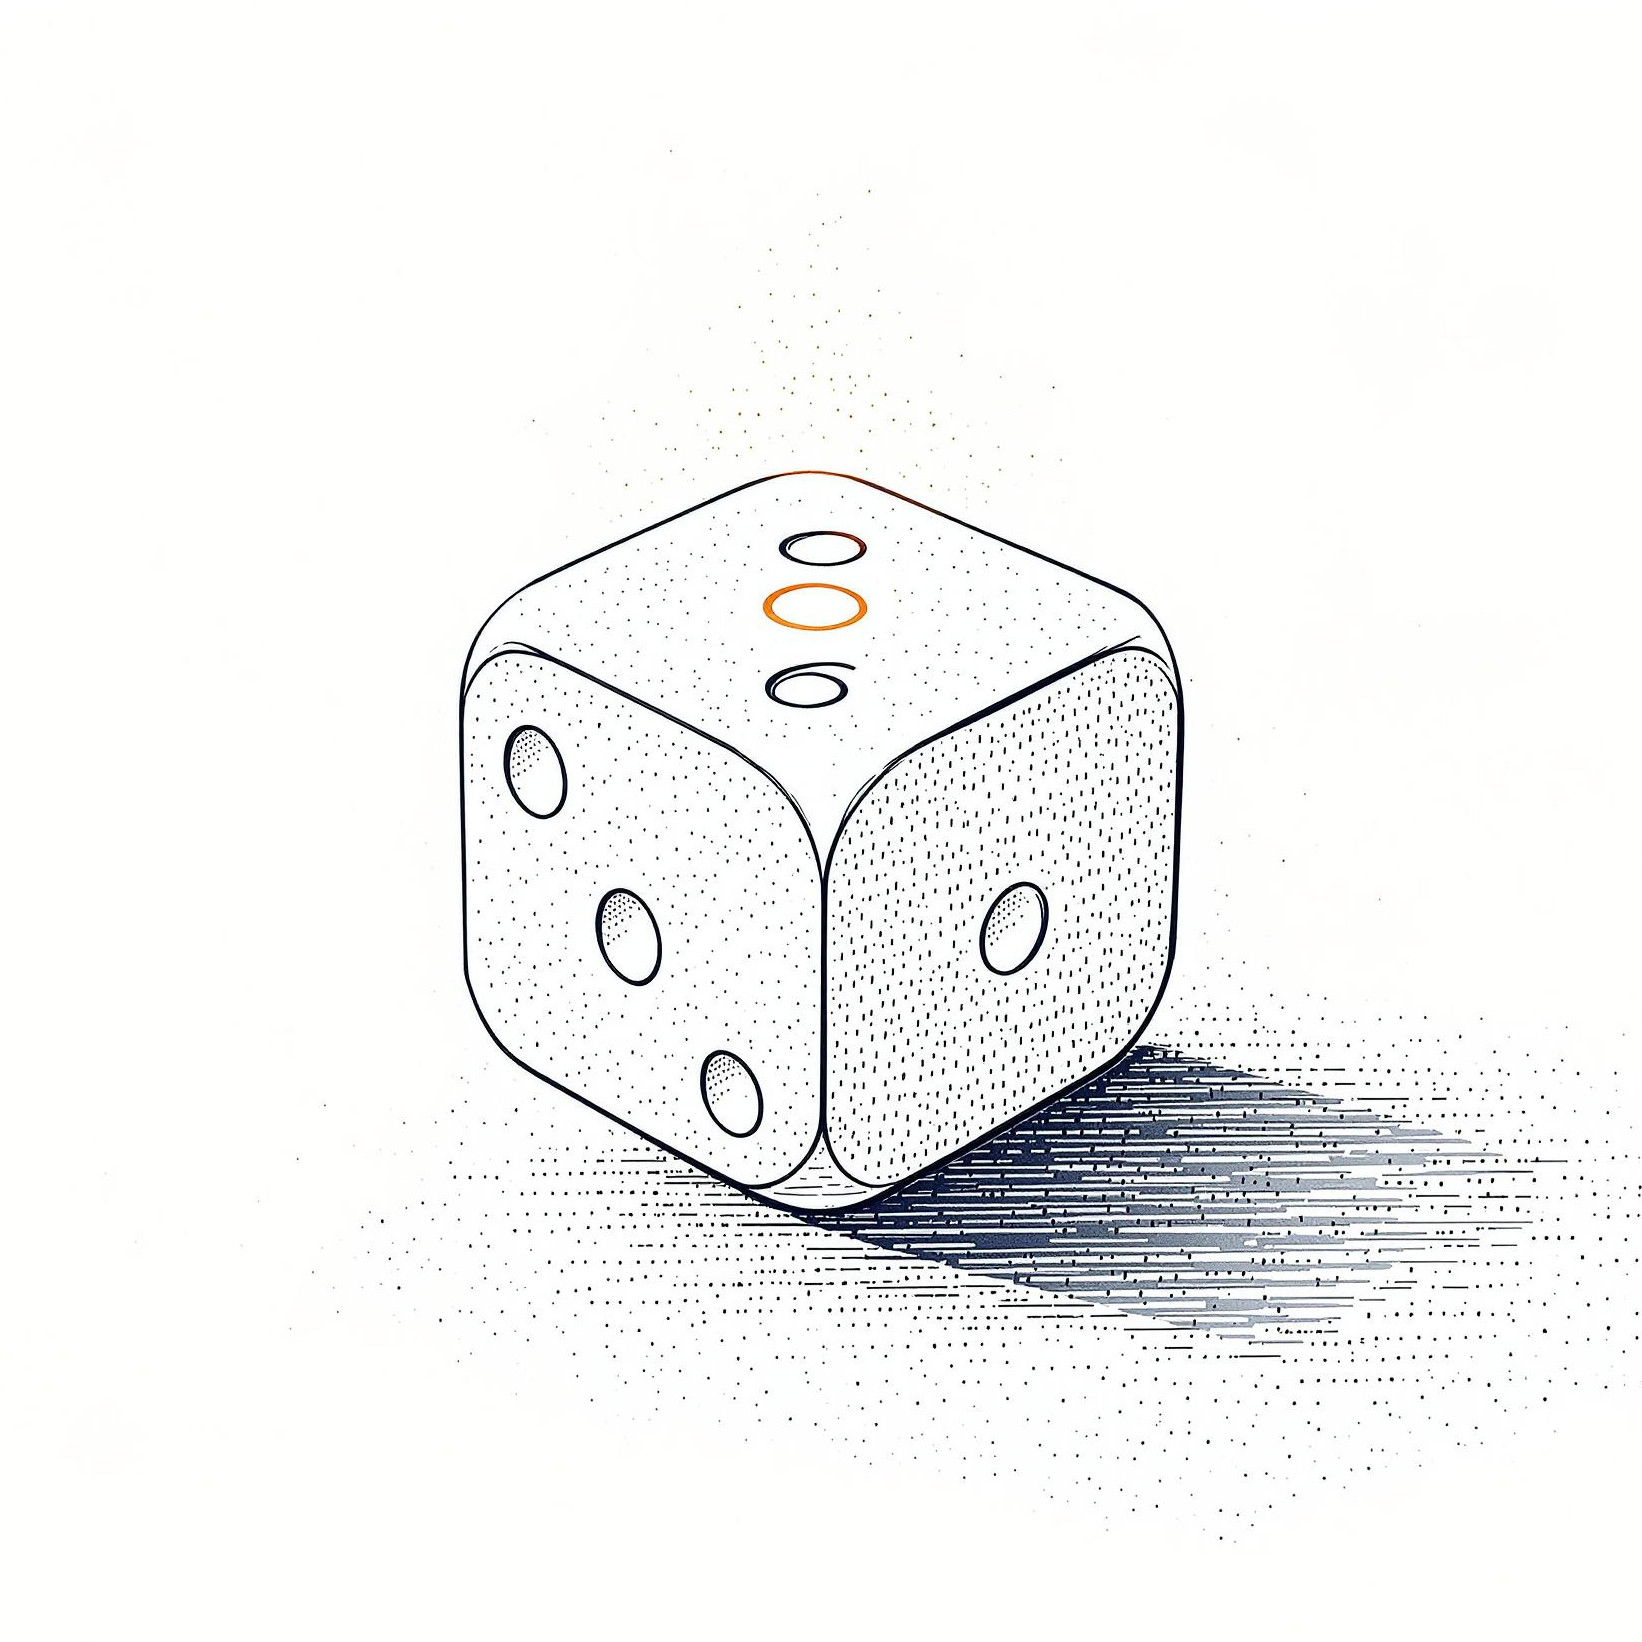
\includegraphics[width=0.4\linewidth]{Documents/250307 BIP Portorož SI/Figures/alea.jpg}
    
            \vspace{1em}
            
            \noindent
            \onslide<4->
                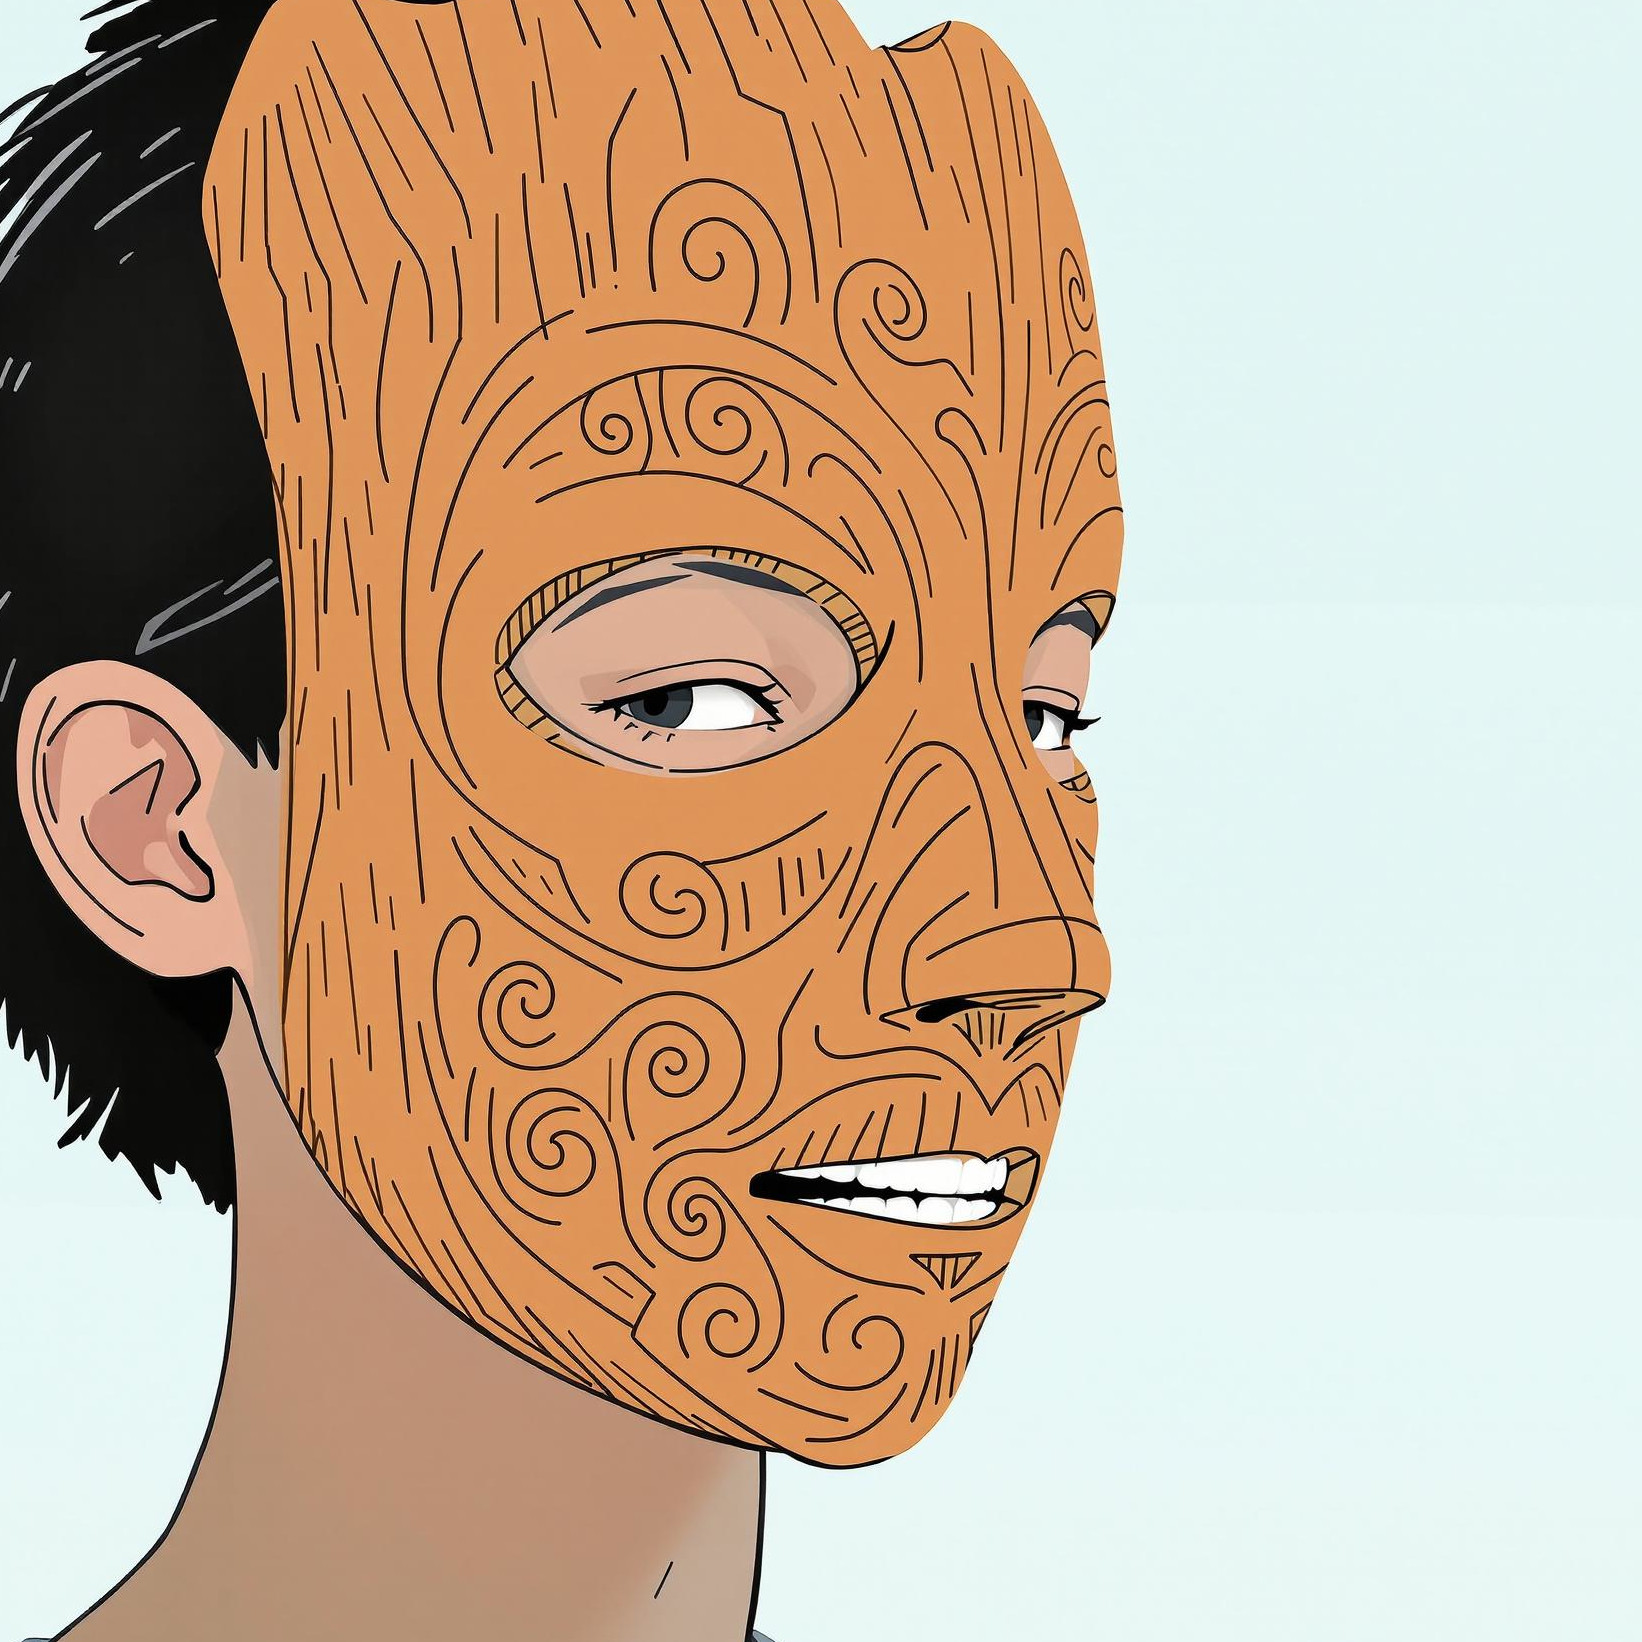
\includegraphics[width=0.4\linewidth]{Documents/250307 BIP Portorož SI/Figures/mimicry.jpg}
            \hspace{1em}
            \onslide<5>
                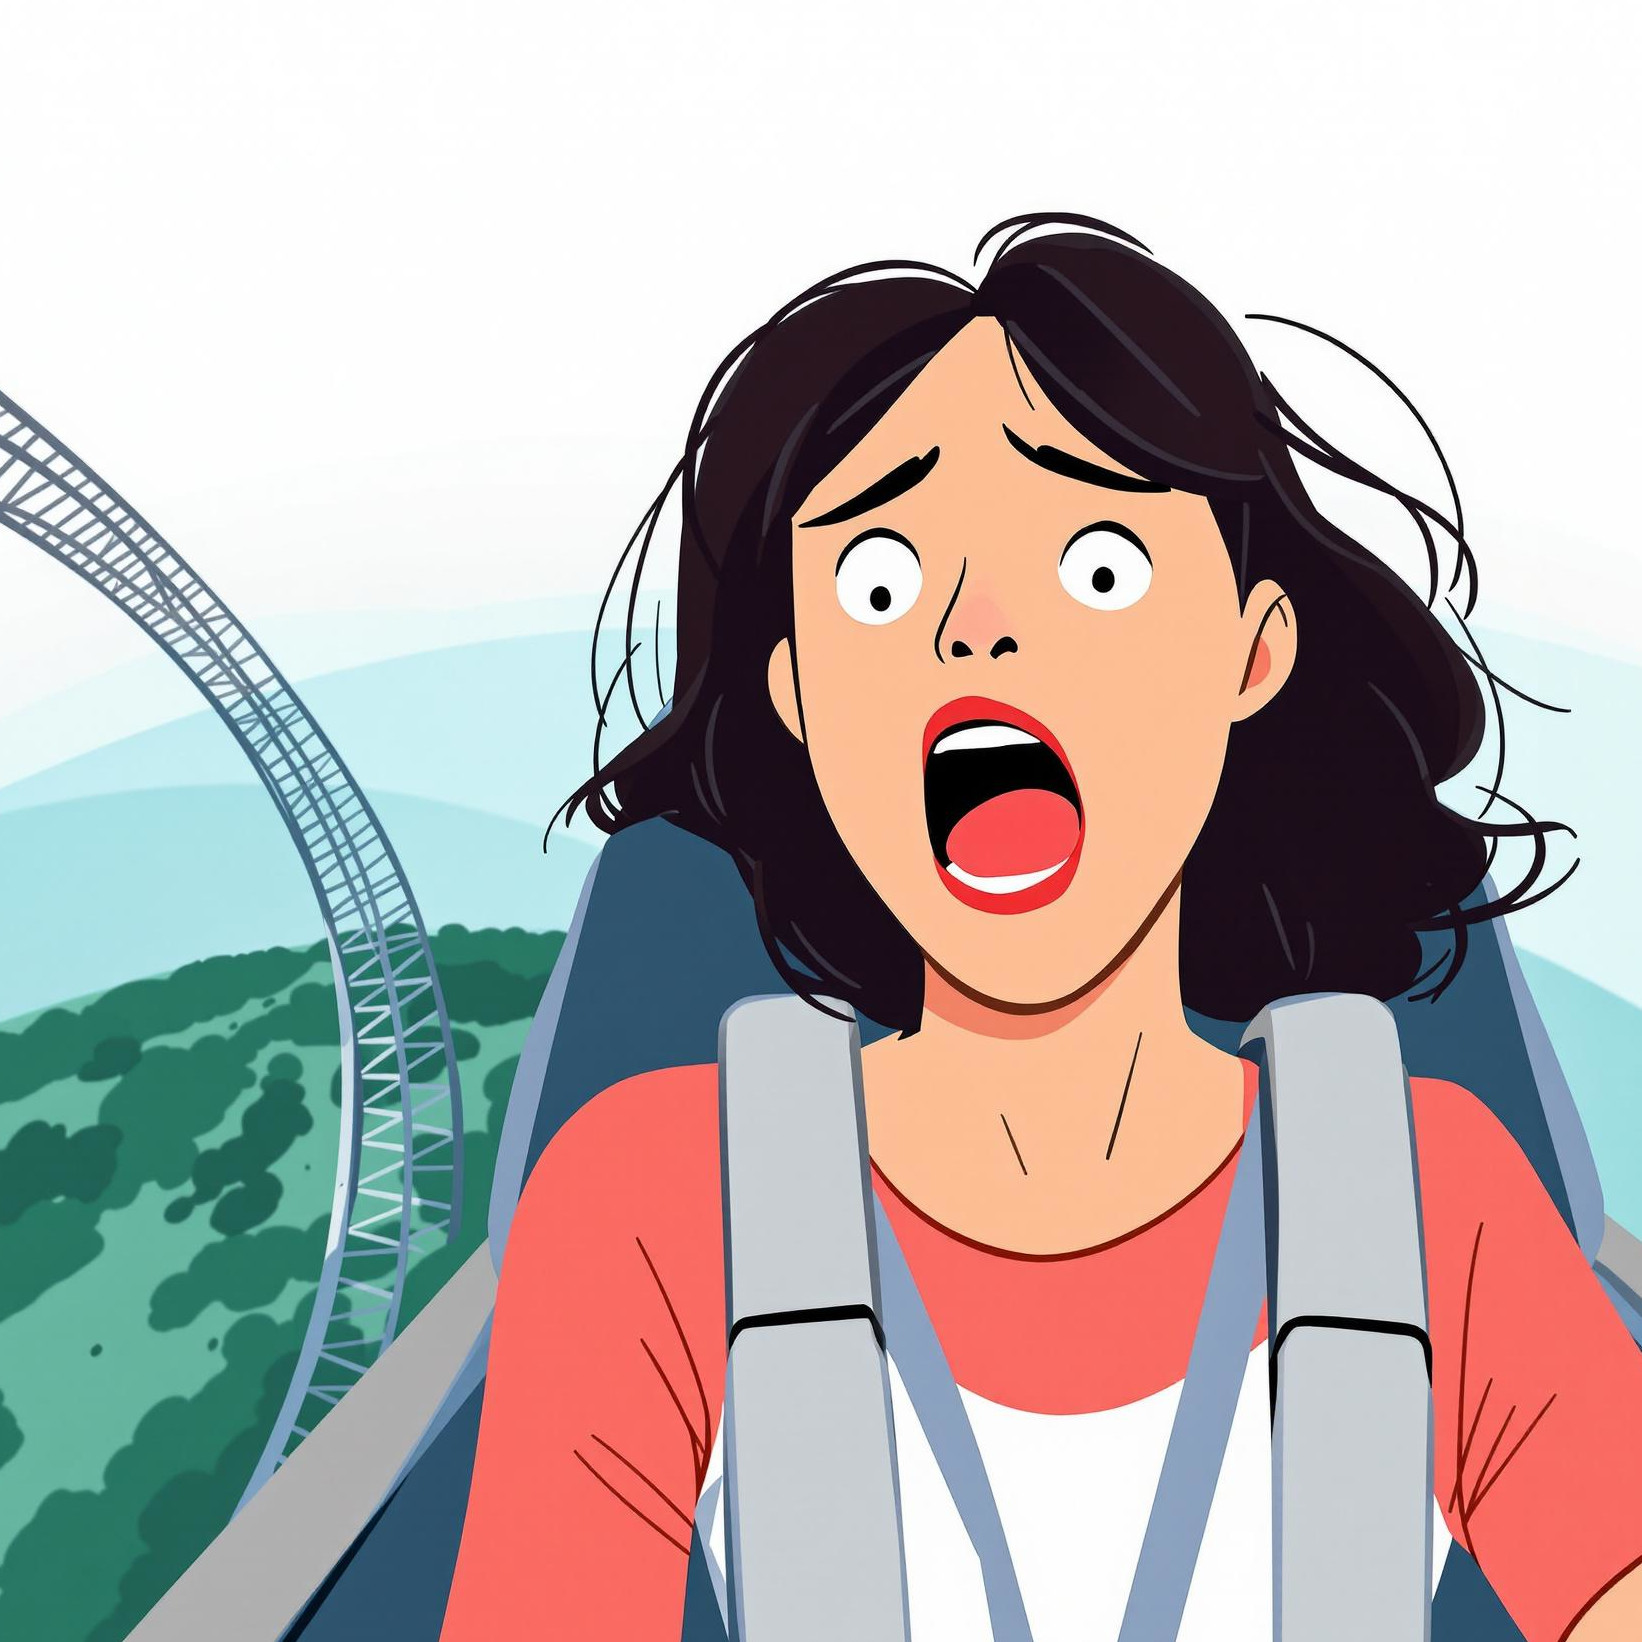
\includegraphics[width=0.4\linewidth]{Documents/250307 BIP Portorož SI/Figures/ilinx.jpg}
        \end{center}

    \end{multicols}
\end{frame}

\begin{frame}[standout]
    \onslide<+->
    \customFigure[0.9]{
        \includegraphics{Documents/250307 BIP Portorož SI/Figures/Mindmap}
    }{Visual representation of knowledge thus far}{Mindmap game}
\end{frame}